\documentclass[12pt, oneside]{article}
\usepackage[letterpaper, margin=1in, headsep=0.5in, left=0.3in, right=2.5in]{geometry}
\usepackage[english]{babel}
\usepackage[utf8]{inputenc}
\usepackage{amsmath}
\usepackage{amsfonts}
\usepackage{amssymb}
\usepackage{tikz}
\usepackage{yhmath}
\usetikzlibrary{quotes, angles}
\usepackage{graphicx}
\usepackage{enumitem}
\usepackage{multicol}

\newif\ifmeta
\metatrue %print standards and topics tags

\title{Regents Geometry}
\author{Chris Huson}
\date{May 2022}

\usepackage{fancyhdr}
\pagestyle{fancy}
\fancyhf{}
\renewcommand{\headrulewidth}{0pt} % disable the underline of the header
\raggedbottom

%\fancyhead[LE]{\thepage}
\fancyhead[RO]{Name:}
\fancyhead[LO]{BECA / Dr. Huson / Geometry Regents Mixed Review}
\cfoot{\thepage}

\begin{document}
\subsubsection*{R.4 Rhombus}
\begin{enumerate}
\item Rhombus diagonal length\\
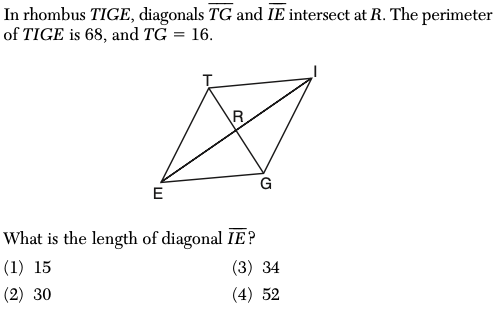
\includegraphics[width=9cm]{R-4images/R-4RhombusH.png}
\vspace{1cm}

\item Rhombus transformations ``onto''\\
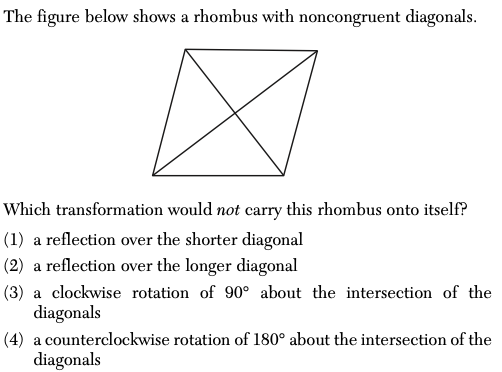
\includegraphics[width=10cm]{R-4images/R-4RhombusF.png}

\item Rhombus side length\\
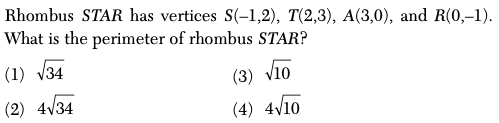
\includegraphics[width=10cm]{R-4images/R-4RhombusE.png}

\newpage
\item Rhombus reflection\\
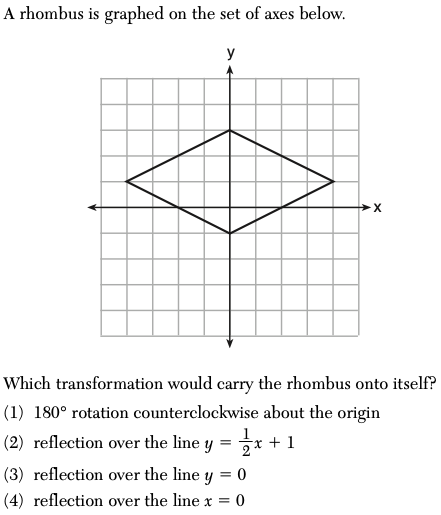
\includegraphics[width=10cm]{R-4images/R-4RhombusJ.png}

\item Rhombus properties (perpendicular diagonals)\\
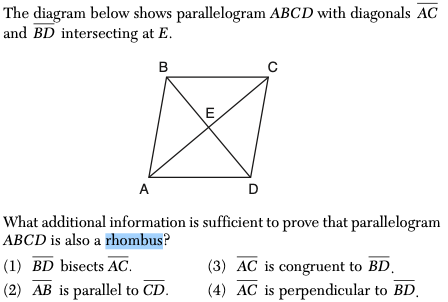
\includegraphics[width=11cm]{R-4images/R-4RhombusD.png}

\newpage
\item Rhombus angle calculation\\
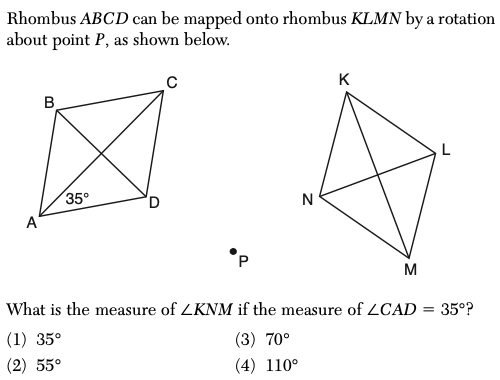
\includegraphics[width=10cm]{R-4images/R-4RhombusK.png}

\item Inscribe angle measures situation\\
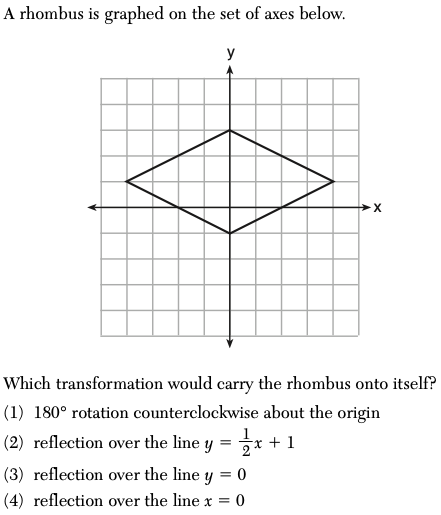
\includegraphics[width=10cm]{R-4images/R-4RhombusJ.png}
\vspace{1cm}

\item Semicircle-inscribed triangle angle measure situation\\
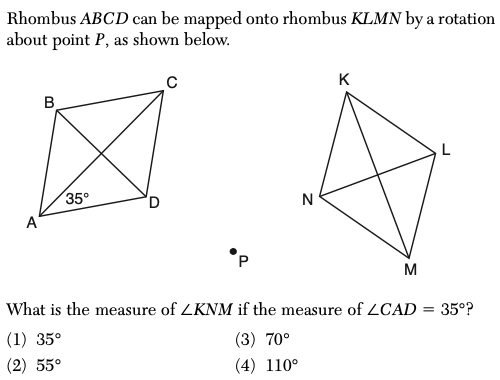
\includegraphics[width=10cm]{R-4images/R-4RhombusK.png}
\vspace{1cm}

\newpage
\item Secant / tangent length situation\\
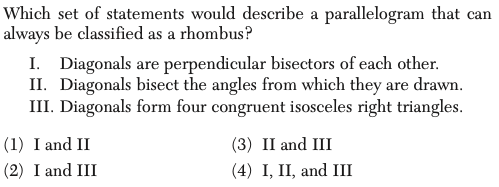
\includegraphics[width=12cm]{R-4images/R-4RhombusA.png}
\vspace{2cm}

\item Secant angle situation\\
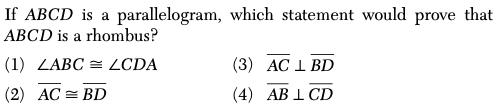
\includegraphics[width=12cm]{R-4images/R-4RhombusB.png}
\vspace{1cm}

\end{enumerate}
\end{document}
  